\section{Evaluation}
\label{sec:validation}

In this section we present the validation of our approach. As aforementioned, this validation is twofold. On one hand, we demonstrate that our approach is correct. To do so, we take use a case study that is well documented in \cite{Crane:2007} and where we exactly know the commonalities existing among the input set. We execute our approach and we compare the results while expecting that the input of our tool matches with the commonalities we know. It is important to mention that this case study corresponds to a real problematic in the industry. Concretely, it is one of the motivations of the VaryMDE\footnote{\url{http://varymde.gforge.inria.fr/}} project which is a collaboration between Thales Research \& Technology, and INRIA.  

The second part of the evaluation is intended to demonstrate that our approach is relevant. We demonstrate, with empirical data, that the phenomenon of syntactic and semantic commonalities is currently appearing in real DSLs and, so, there is an important amount of potential reuse in the wild and our approach can be actually useful. 

\subsection{Evaluating \textit{correctness}: The state machines case study}

The case study is composed of three different DSLs for expressing state machines:  UML state diagrams \cite{UML:2011}, Rhapsody \cite{Harel:2004}, and Harel's state charts \cite{Harel:1996}. Because the three DSLs are intended to express the same formalism, they have commonalities. For example, all of them provide basic concepts such as \texttt{StateMachine}, \texttt{State}, \texttt{Transition}, or \texttt{Trigger}. However, not all those DSLs are equal. In fact, they have some syntactic and semantic differences which are well documented in the Crane's article \cite{Crane:2007}. To validate our approach we implemented these three DSLs while strictly following that documentation. Thus, we obtained a set of DSLs to test our tool and we know in advance the results that the tool should provide. We use that as an oracle to test our approach. 

\subsubsection{Oracle.} Figure \ref{fig:oracle} shows a table with the constructs contained by each DSL in the case study. Note that not all the DSLs have exactly the same constructs. The main differences are in the support for types of triggers. Whereas Rhapsody only supports simple triggers. Harel's state charts and UML provide support composing triggers. In particular, in Harel's state charts triggers can be composed by using \texttt{AND}, \texttt{OR}, and \texttt{NOT} operators. In turn, in UML triggers can be composed by using only the \texttt{AND} operator. Another difference between the DSL of our case study corresponds to the different support for pseudostates. Whereas there are pseudostates that are supported by all the DSLs (\texttt{Fork}, \texttt{Join}, \texttt{ShallowHistory}, and \texttt{Junction}); there are certain psueudostates such as \texttt{DeepHistory}, \texttt{Conditional}, or \texttt{Choice} that are not supported in all of the DSLs.

\begin{figure}
\centering
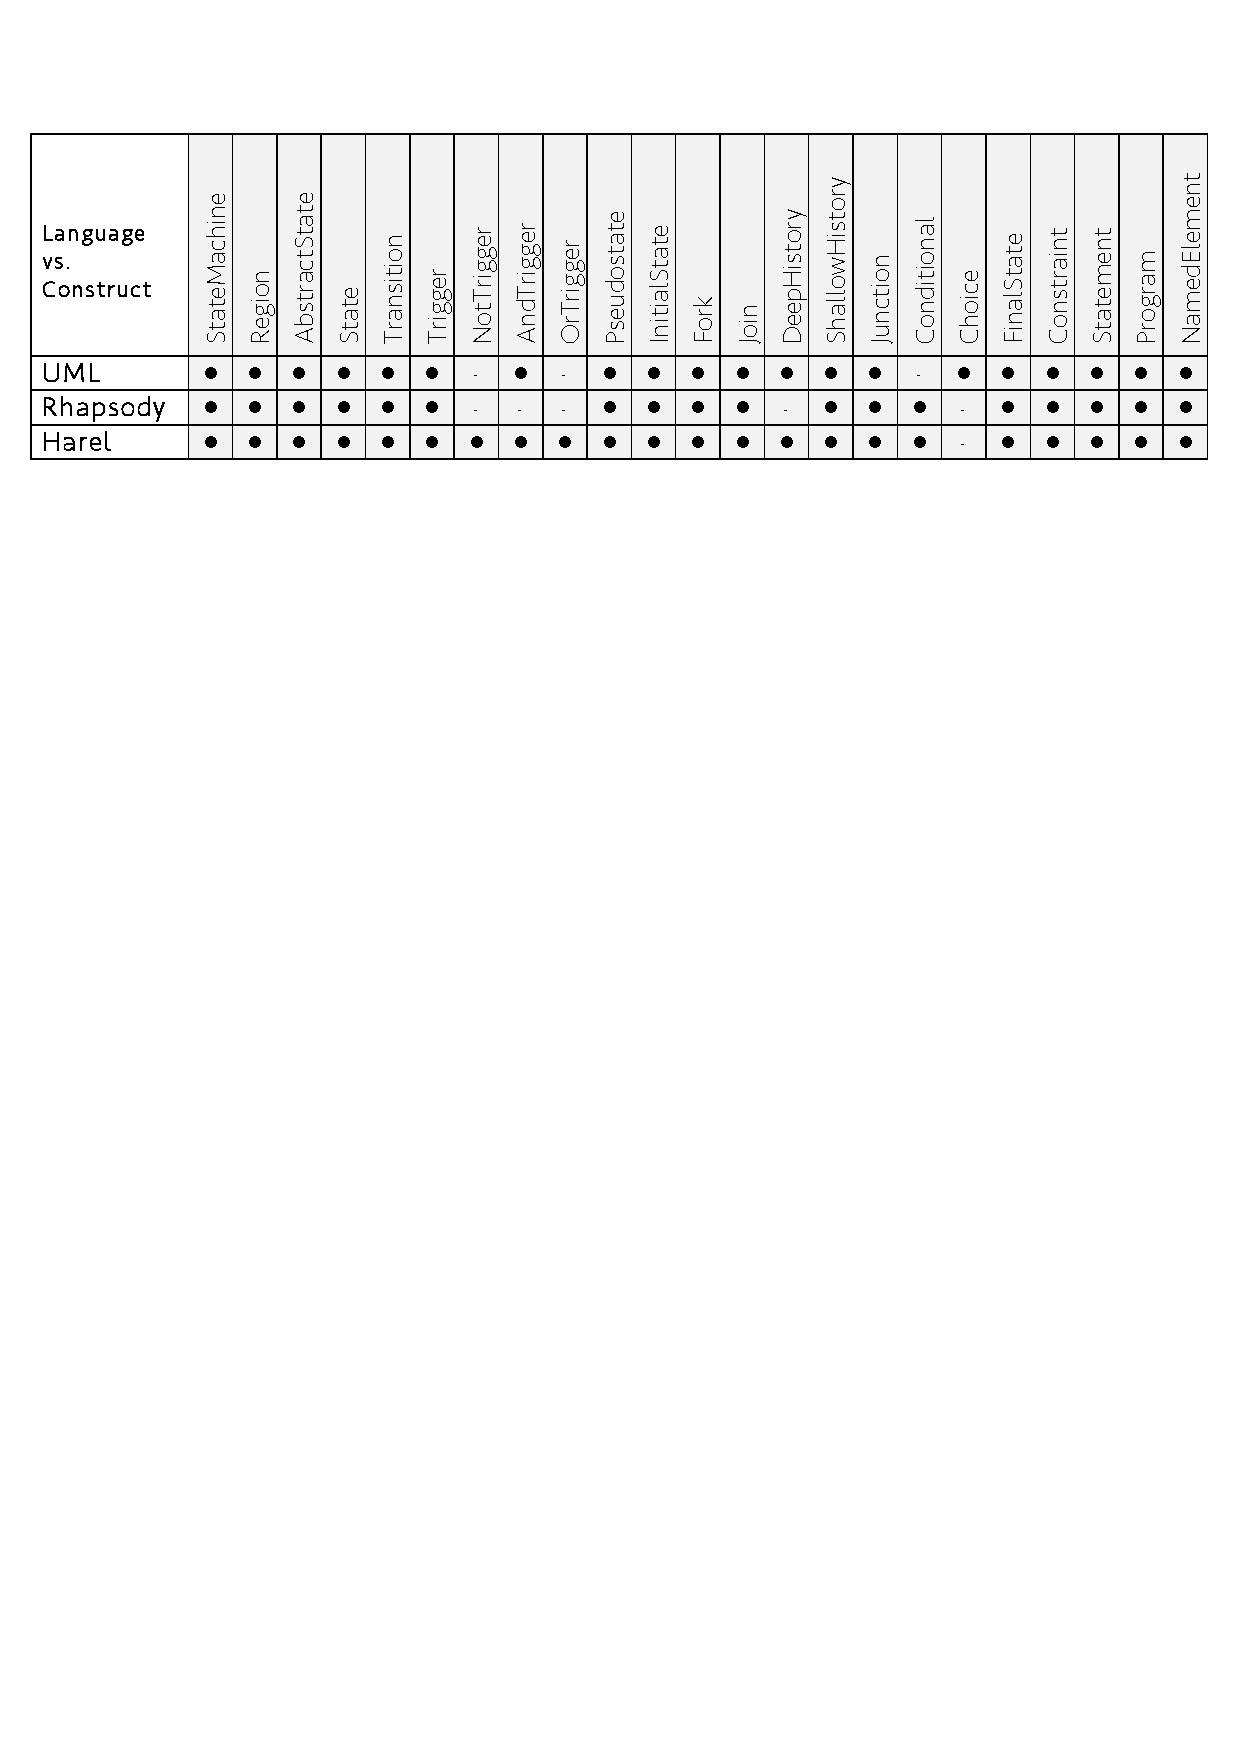
\includegraphics[width=1\linewidth]{images/oracle.pdf}
\caption{Oracle for evaluation of correctness}
\label{fig:oracle}
\end{figure}

In summary, there are: 17 language constructs that are shared by all the DSLs; 1 construct that is exclusive of UML, 2 constructs that are exclusive of Harel's state charts; 2 constructs shared by UML and Harel's state charts; and 1 construct shared by Harel's state charts and Rhapsody. 

\vspace{-2mm}
\subsubsection{Results.} Figure \ref{fig:puzzle-overlapping} shows the results of the first part of the analysis. It presents the Venn diagram produced for the case study of the state machines. Note that the numbers correspond to our oracle demonstrating that our approach is correct. Due to lack of space, we do not present the semantic results. However, in a later section we present a tool demonstration that shows the complete functionality of our tool.

\begin{figure}
\centering
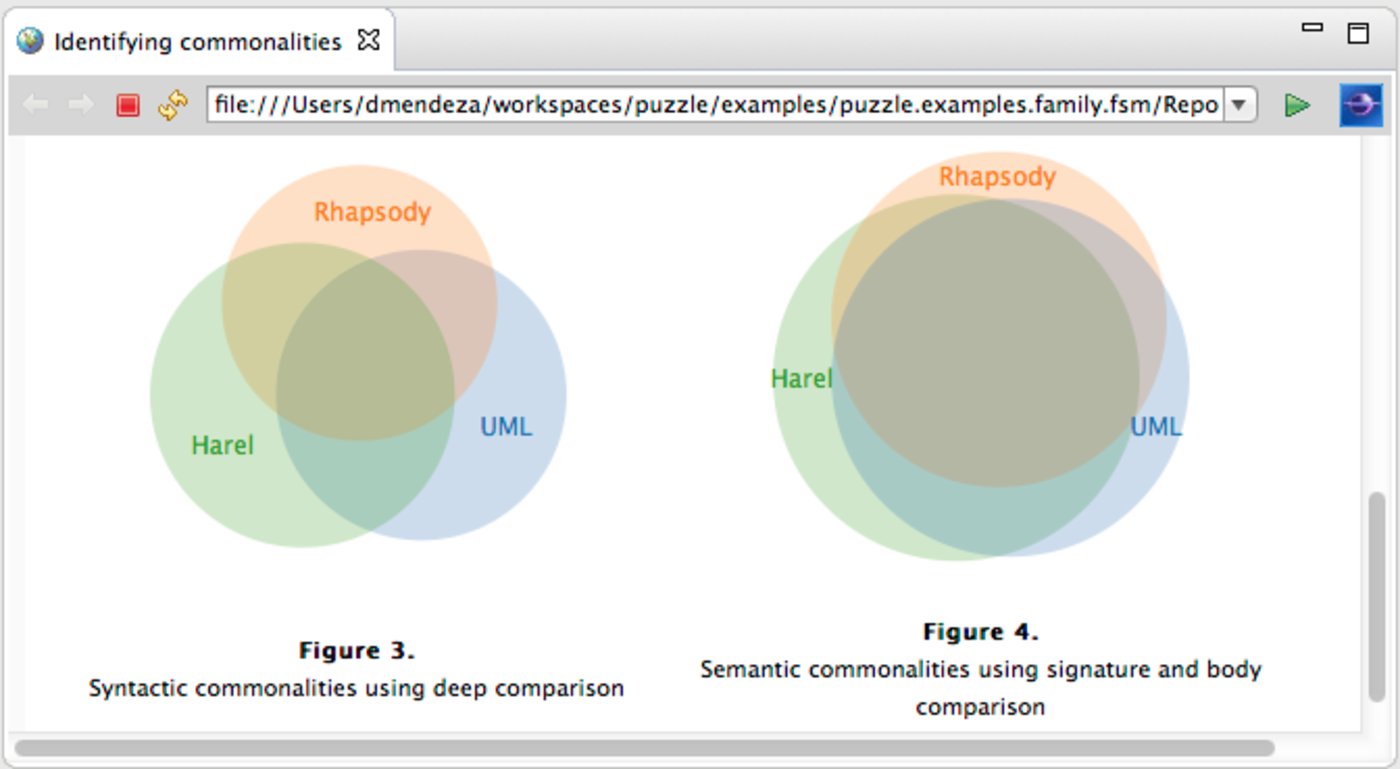
\includegraphics[width=1\linewidth]{images/puzzle-overlapping.pdf}
\caption{Results for the state machines case study: identifying overlapping}
\label{fig:puzzle-overlapping}
\end{figure}

Figure \ref{fig:puzzle-modularization} shows the results for the second and third part of our approach: identifying and extracting reusable language modules. Note that there is a language module (core) that contains all the language constructs that are shared by the three DSLs. Then, the other language modules encapsulate pseudostates and triggers separately since they represent the differences among the DSLs. Note that in order to obtain the Harel's state charts language, we need to compose the modules 1, 2, and 5. In turn, to obtain UML we need to compose modules 1, 3, and 4. Finally, to obtain Rhapsody we need to compose modules 1 and 5.

\begin{figure}
\centering
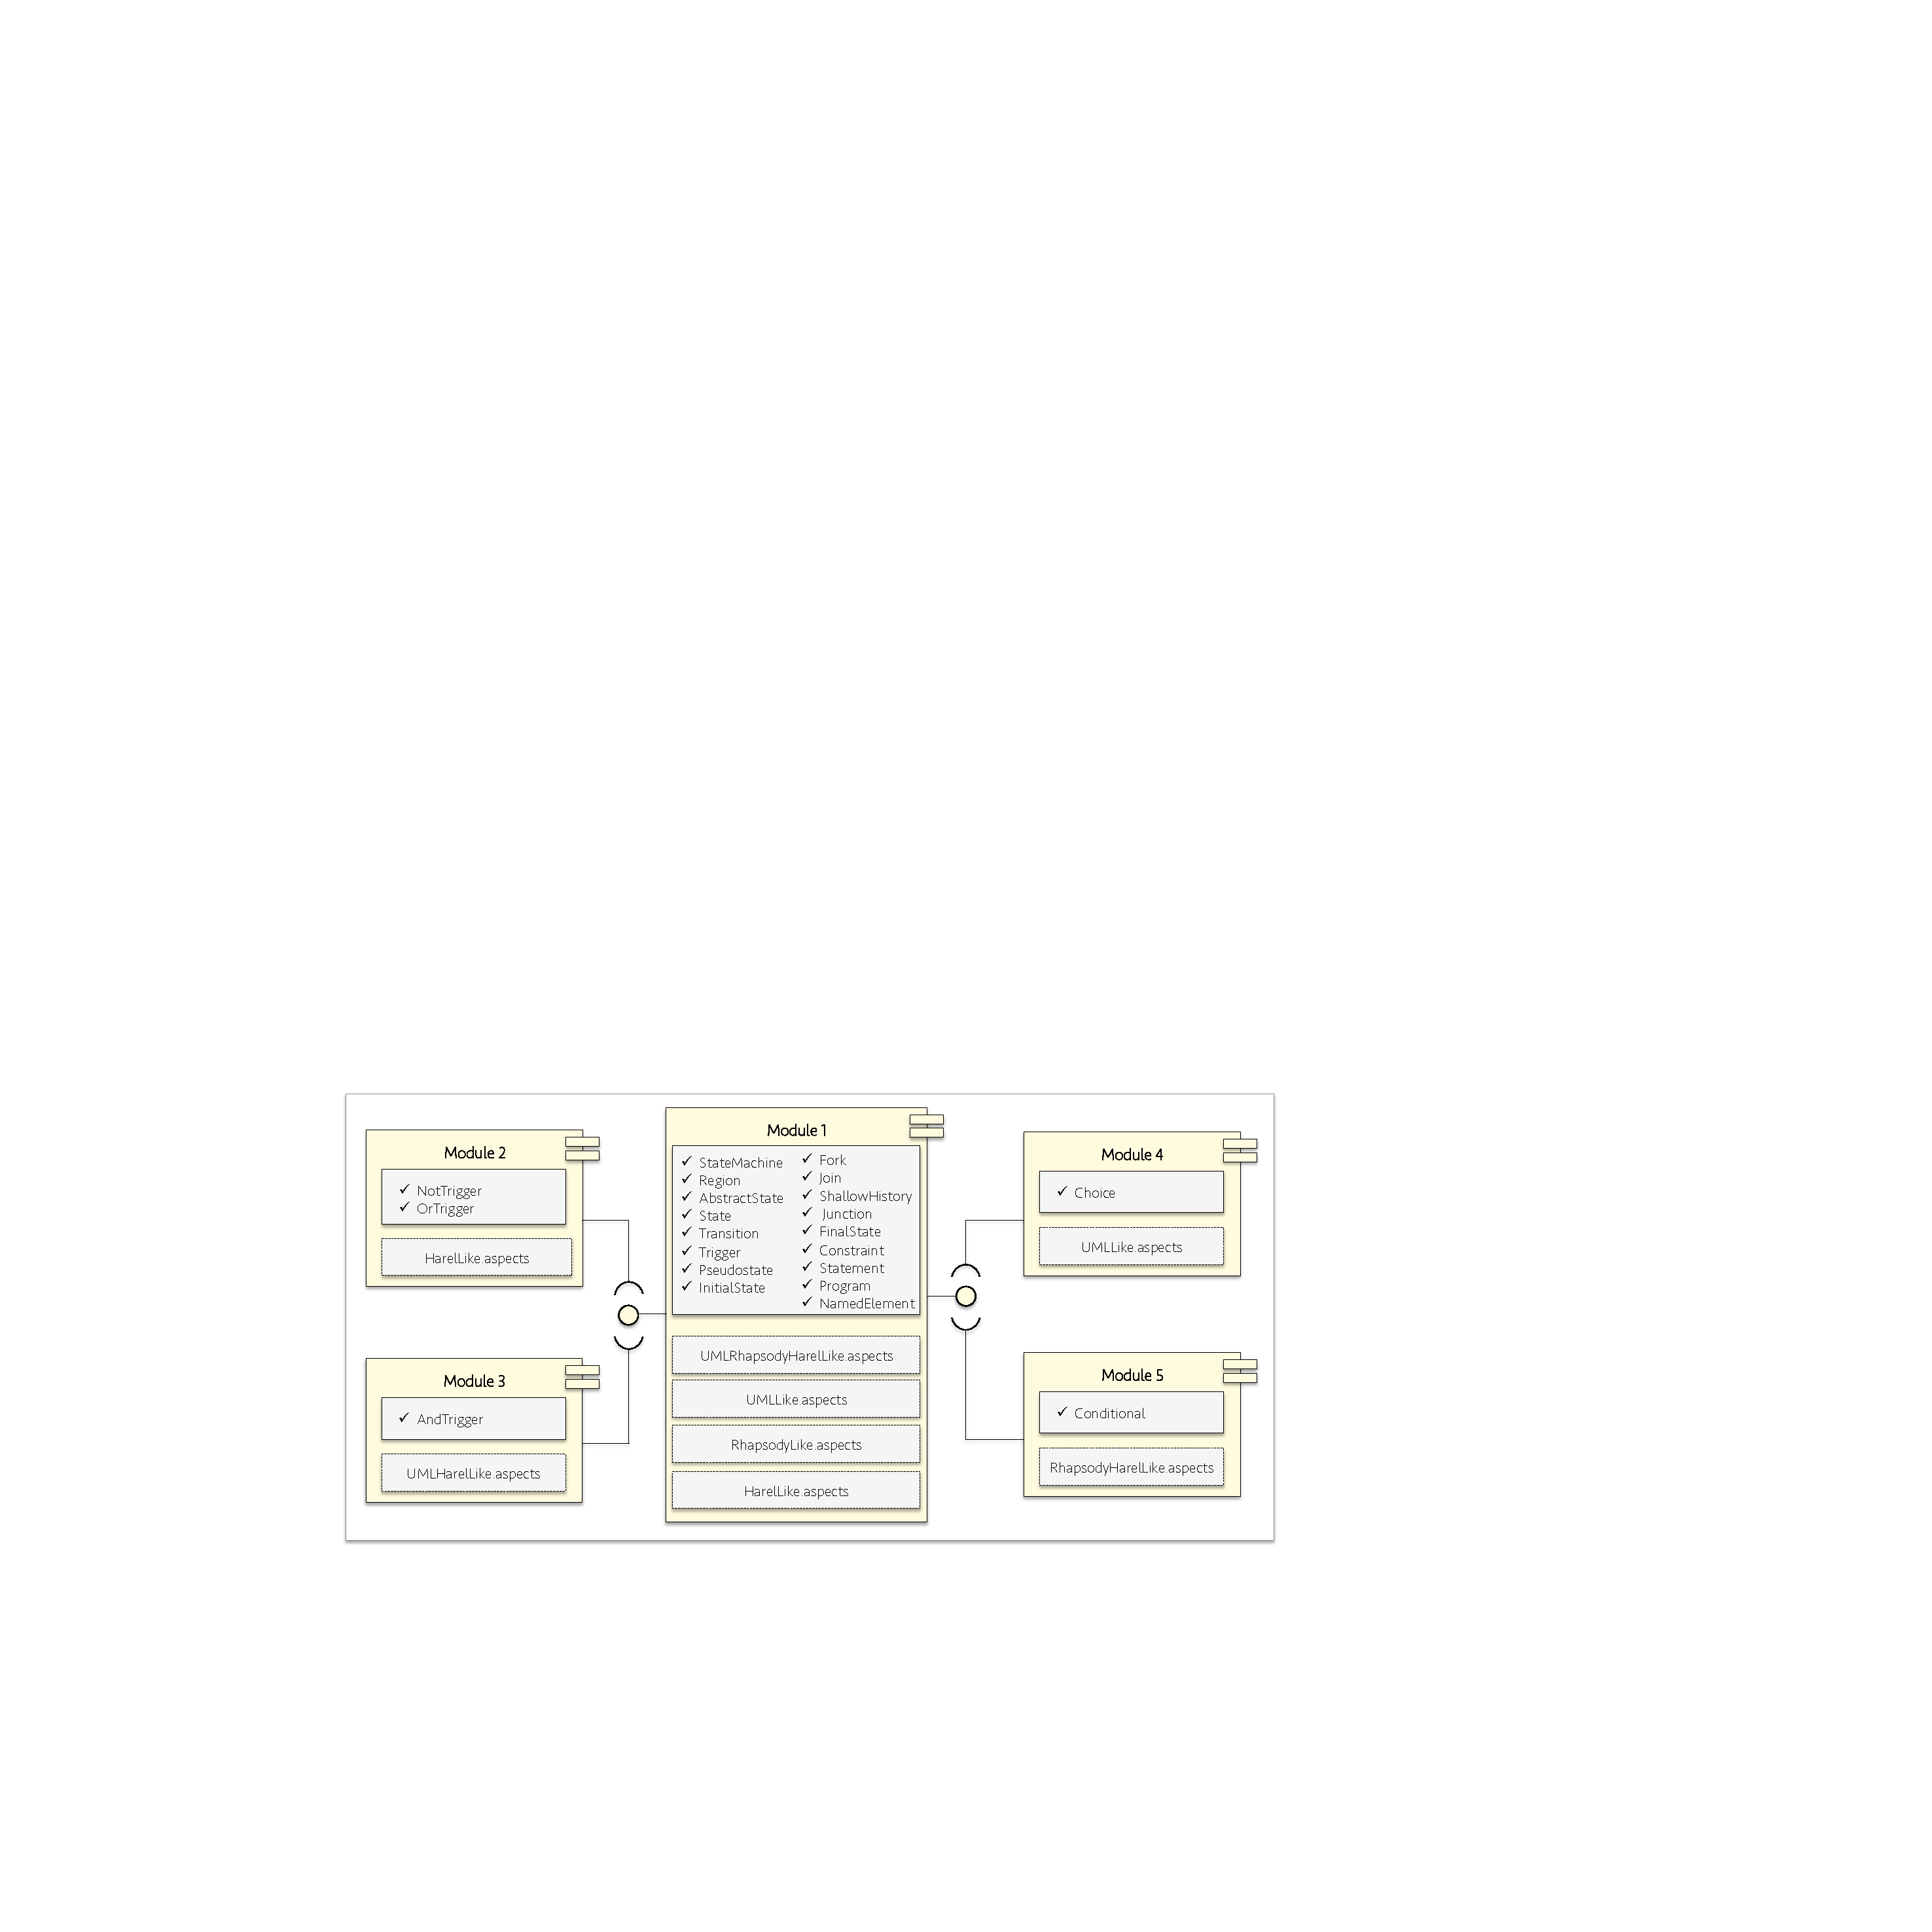
\includegraphics[width=1\linewidth]{images/puzzle-modularization.pdf}
\caption{Results for the state machines case study: extracting language modules}
\label{fig:puzzle-modularization}
\end{figure}

\subsection{Evaluating \textit{relevance}: Identifying potential reuse in the wild}

In order to identify potential reuse in the wild, we explored the public \texttt{GitHub} repositories in search of DSLs that are built on the same technological space that we used in our approach. Namely, metamodels written in Ecore with operational semantics defined in Xtend as domain-specific actions. The objective was to build a data set composed of DSLs developed by diverse development teams. 

As a result of this search, we found 2800 Ecore metamodels after discarding metamodels with errors. Contrariwise, due to the fact that Kermeta 3 and its implementation in Xtend is a quite recent idea, we only found some few DSLs all of them developed in our research team (which is the team that developed Kermeta 3). We decided to conduct analysis only in the metamodels. We consider that such analysis a good insight to know if there is potential reuse.

\subsubsection{The questions.} Our analysis to evaluate potential reuse in the wild was guided by two questions: 1) What is the probability that a metamodel share some commonalities with another one? and 2) How big is the average commonality between metamodels?

\subsubsection{The experiments.} In order to answer the first question, we conducted an experiment intended to compute the number of metamodels that share at least one construct with another metamodel. In other words, we consider our data set as a data sample in order to predict the probability that a metamodel share commonalities with another one. To do that, we 

one was intended to know what is the average of metamodels to which a metamodel share something. To do so, we execute a pair-wise analysis between all the metamodels and compute a matrix. 

\subsubsection{The answers.}

The experiments were conducted using a version of \toolname implemented in Java. Further, \toolname was installed in the Grid5000 Cloud, which is a cluster with more than 5000 cores from were we took XX dual-CPU Dell Blades with Intel Xeon X3470 CPUs running at 2.93GHz, with 16 threads 
per CPU, and CentOS v6. Each dual-CPU Dell Blade has 36GB of RAM. 

\subsection{Tool demonstration}
\label{sec:tooldemo}

The tooling supporting the approach presented in this paper is implemented on top of the Eclipse Modeling Framework. We provide a tool demonstration\footnote{Tool demonstration: \url{www.tooldemo.com}} that illustrates the use of our tool in both: the example presented in section \ref{sec:motivation} and the case study of the state machines presented in section \ref{sec:validation}.


%\begin{table*}[htbp]
%  \centering
% \scalebox{0.8}{
%\begin{tabular}{|p{0.2\textwidth}|p{0.3\textwidth}p{0.1\textwidth}p{0.4\textwidth}|}
%\hline
%\multicolumn{4}{|c|}{\textbf{Hypotheses of Experiment 1}} \\ \hline
%\textbf{Null Hypothesis ($H_0$)} & \multicolumn{ 3}{|p{0.8\textwidth}|}{\toolname is capable of detecting %commonalities in the case study that motivated this research.} \\ \hline
%\textbf{Alt. Hypothesis ($H_1$)} & \multicolumn{ 3}{|p{0.8\textwidth}|}{
%\toolname is not capable of detecting commonalities in the case study that motivated this research.} \\ %\hline
%\textbf{Dependent variable} & \multicolumn{ 3}{|p{0.8\textwidth}|}{The set of ecores representing our %languages. }\\ \hline
%\textbf{Blocking variables} & \multicolumn{ 3}{|p{0.8\textwidth}|}{The most sold phones and the market %share indexes. }\\ \hline
%\textbf{Model used as input} & \multicolumn{ 3}{|p{0.8\textwidth}|}{\textit{models in %\url{urlhacialosmodelos}} }
%\\
%\hline \hline


%\multicolumn{4}{|c|}{\textbf{Hypotheses of Experiment 2}} \\ \hline
%\textbf{Null Hypothesis ($H_0$)} & \multicolumn{ 3}{|p{0.8\textwidth}|}{The use of \toolname 
%will not result in a higher market-share impact metric than selecting the most commonly sold 
%phones, for a given maximum budget.} \\ \hline
%\textbf{Alt. Hypothesis ($H_1$)} & \multicolumn{ 3}{|p{0.8\textwidth}|}{The use of \toolname 
%will result in a higher market-share impact metric than selecting the most commonly sold 
%phones, for a given maximum budget.}\\ \hline
%\textbf{Model used as input} & \multicolumn{ 3}{|p{0.8\textwidth}|}{\textit{Android feature model presented %in Figure \ref{fig:featureModel}} }\\ 
%\hline
%% @J - Do you mean independent?! My understanding is that a blocking variable is a grouping variable...
%\textbf{Blocking variables} & \multicolumn{ 3}{|p{0.8\textwidth}|}{The most sold phones, market share %indexes and the maximum cost allowed set to 600\$. }\\ \hline
%\textbf{Model used as input} & \multicolumn{ 3}{|p{0.8\textwidth}|}{\textit{Android feature model presented in Figure \ref{fig:featureModel}} }\\
%\hline \hline

%\multicolumn{4}{|c|}{\textbf{Constants}} \\ \hline
%\textbf{CSP solver} & \multicolumn{ 3}{|p{0.8\textwidth}|}{\textit{ChocoSolver v2} } \\ \hline
%\textbf{Heuristic for variable selection in the CSP solver} & \multicolumn{ 3}{|p{0.8\textwidth}|}{\textit{Default}}\\
%\hline 

%\hline 
%\end{tabular}%
%}
%\caption{Hypotheses and design of experiments.}
%  \label{tab:Exp1aDesign}
%\end{table*}
%\todo{poner la tabla para con los datos de los experimentos que vamos a ejecutar/hemos ejecutado. Intenta pensar cuales pueden ser las conclusiones que quieres extraer. Yo propongo 3 abajo.}

%Table \ref{tab:Exp1aDesign} shows the hypothesis of the experiments executed to validate our 
%approach. To make the experiments reproducible, a number of fixed assumptions are made, such as homogeneous feature costs. ChocoSolver 
%\footnote{\url{http://www.emn.fr/z-info/choco-solver/}}, with it's default heuristic, is 
%used as the CSP solver for extracting software products from the feature model presented 
%in Figure \ref{fig:featureModel}

%\textbf{Technological space and experimental platform:} Currently, there are diverse techniques available for the implementation of syntax and semantics of DSLs \cite{Mernik:2005b}. Language designers can, for example, choose between using context-free grammars or metamodels as specification formalism for syntax. Similarly, there are at least three methods for expressing semantics: operationally, denotationally, and axiomatically \cite{Mosses:2001}. In this paper we are interested on DSLs which syntax is specified by means of metamodels and semantics is specified operationally as a set methods (a.k.a, \textit{domain-specific actions} \cite{Combemale:2013}). Each language construct is specified by means a metaclass and the relationship between language constructs are specified as references between metaclasses. In turn, domain-specific actions are specified as java-like methods that are allocated in each metaclass.
